\documentclass[10pt,a4paper]{article}
\usepackage[margin=18mm]{geometry}
\usepackage{amsmath,booktabs,longtable,graphicx,hyperref}
\title{Longer CSA feedback retention for NAUSICA}
\date{\today}
\begin{document}\maketitle
\section{Circuit and physical inputs}
The scan extends the existing 180 nm circuit by varying the feedback transistor
length. Its width is 0.36 $\mu$m and its gate is grounded. The external input
capacitance is 1.25 pF, the feedback capacitance is 3 fF and the supply is 1.8 V
at 20 $^\circ$C. The amplifier dimensions and other biases are held fixed.
The M4 bias is selected to restore the reference quiescent output and rounded
to four decimal places. These are transistor-model calculations.

The physical input is the established on-axis benchmark: a 0.5 mm square pad in
an infinite grounded plane, with pad weighting potential one and all other
boundaries, including infinity, zero. The dielectric is homogeneous. Ions
approach at constant speed 3 m/s through a finite 5 mm gap and are collected
uniformly within the specified frame. The input integral per ion remains
$e[1-\phi_w(g)]$; no extra collection impulse or charge renormalization is added.
The stored event histories use the corrected direct carrier collection.

\section{Discharge calibration and measurement}
Independent zero-current transients establish the baseline. Ten- and hundred-ion
packets provide six-second tails. Exponential fits are checked against a finer
solver grid, three tail intervals and the two charge amplitudes.
For the fitted $\tau$, $\alpha=\exp(-\Delta t/\tau)$ and the measured signal is
$D_n=-(\overline V_n-\alpha\overline V_{n-1})$ relative to the baseline.
Each voltage uses a centred 5 ms average. The small-signal gain is calibrated
with 100 ions and checked through 2000 ions.

SPICE supplies the one-sided output noise spectrum. Julia integrates the spectrum
with the averaging and frame-difference transfer function from 0.0001 Hz to
1 MHz. Lower bounds of 0.001 and 0.1 Hz are also saved. Two spectral densities,
two quadrature orders and two transient resolutions check convergence.
The 400 $\mu$m feedback device gives 46.04 and 51.38 electrons RMS for 20 and 40 ms frames in the extended noise band.
\begin{center}\small
\begin{tabular}{rrrrrrrr}\toprule
$L_f$ & M4 bias & $V_0$ & $\tau$ & ENC (20 ms) & ENC (40 ms) & $g_{20}$ & $g_{40}$\\
($\mu$m) & (V) & (V) & (s) & ($e^-$ RMS) & ($e^-$ RMS) & ($\mu$V/ion) & ($\mu$V/ion)\\\midrule
3000 & 0.6903 & 0.873 & 28.23 & 46.04 & 51.38 & 41.00 & 42.35 \\
4000 & 0.6962 & 0.893 & 30.20 & 45.30 & 50.07 & 41.14 & 42.50 \\
\bottomrule\end{tabular}\end{center}
\begin{figure}[ht]\centering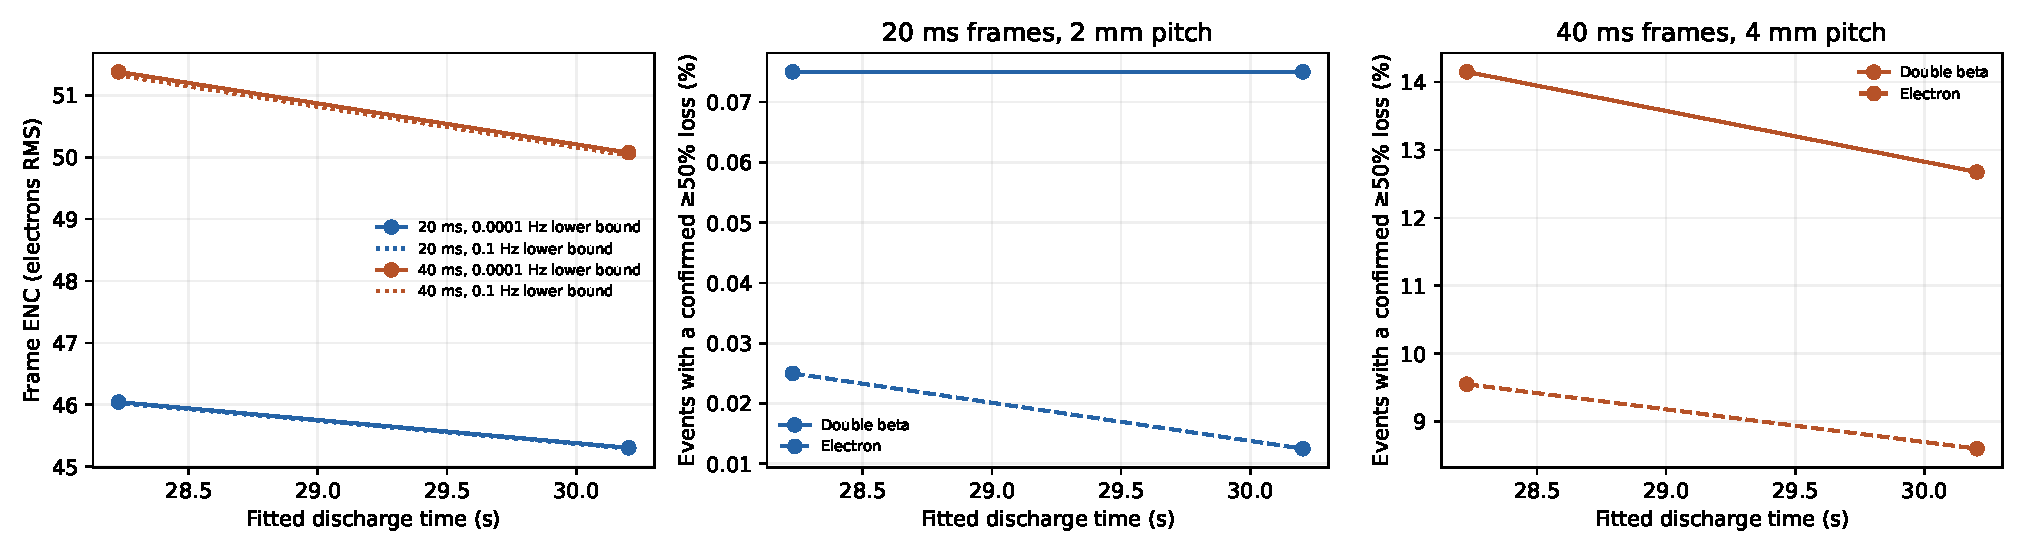
\includegraphics[width=\linewidth]{retention_comparison.pdf}
\caption{Frame noise and confirmed local compression versus fitted retention.
The lower-frequency comparison uses the same spectrum and frame estimator.
Compression flags require a missing signal of at least one nominal frame ENC.}
\end{figure}

\section{Full-history compression}
All stored pad histories, including empty buckets, are screened with the
calibrated linear response. Histories with predicted output below 0.35 V are
simulated nonlinearly in LTspice, together with 12 fixed-seed controls in each
higher-voltage stratum. Each sample contains 8000 events. The 2 mm histories
use 20 ms frames and the 4 mm histories use 40 ms frames.
An event is counted once when a tested pad has a positive-count bucket whose
nonlinear response loses the selected fraction and at least one nominal ENC.
These fractions count confirmed local distortions within the screening study.
Electronic noise is used to set the deficit criterion; random noise is not
added to the mean transients. Event usefulness is assessed with track reconstruction.
\begin{center}\scriptsize
\begin{longtable}{rlrrrrr}\toprule
$L_f$ ($\mu$m) & Sample & Pads simulated & Events & $\geq25\%$ & $\geq50\%$ & $\geq75\%$\\\midrule
3000 & p2\_bb0nu & 66 & 8000 & 0.125 & 0.075 & 0.025 \\
3000 & p2\_electrons & 60 & 8000 & 0.062 & 0.025 & 0.013 \\
3000 & p4\_bb0nu & 3500 & 8000 & 23.275 & 14.150 & 5.838 \\
3000 & p4\_electrons & 2363 & 8000 & 15.937 & 9.550 & 4.188 \\
4000 & p2\_bb0nu & 61 & 8000 & 0.125 & 0.075 & 0.013 \\
4000 & p2\_electrons & 58 & 8000 & 0.037 & 0.013 & 0.013 \\
4000 & p4\_bb0nu & 2977 & 8000 & 20.575 & 12.675 & 5.188 \\
4000 & p4\_electrons & 1979 & 8000 & 14.050 & 8.600 & 3.775 \\
\bottomrule\end{longtable}\end{center}

\section{Noise and compression}
Extending the discharge time from 28.23 to 30.20 s lowers the 20 ms frame ENC from 46.04 to 45.30 electrons RMS, and the 40 ms frame ENC from 51.38 to 50.07. M2 supplies 58.5\% and 54.1\% of the noise variance at the longest retention. For double-beta events, the confirmed 50\% local-loss rate changes from 0.075\% to 0.075\% with 2 mm pads, and from 14.15\% to 12.68\% with 4 mm pads.

\section{Transistor noise budget}
The entries are contributions to the recovered charge; independent transistor
noise variances add. Percentages refer to the total variance.
\begin{center}\scriptsize\begin{longtable}{rrlrr}\toprule
$L_f$ ($\mu$m) & Frame (ms) & Device & ENC contribution & Variance (\%)\\\midrule
3000 & 20 & m1 & 12.67 & 7.58 \\
3000 & 20 & m2 & 34.64 & 56.59 \\
3000 & 20 & m3 & 19.92 & 18.72 \\
3000 & 20 & m4 & 8.90 & 3.74 \\
3000 & 20 & m5 & 0.00 & 0.00 \\
3000 & 20 & m6 & 2.71 & 0.35 \\
3000 & 20 & mf & 16.62 & 13.03 \\
3000 & 40 & m1 & 14.07 & 7.50 \\
3000 & 40 & m2 & 36.81 & 51.32 \\
3000 & 40 & m3 & 21.16 & 16.97 \\
3000 & 40 & m4 & 9.45 & 3.38 \\
3000 & 40 & m5 & 0.00 & 0.00 \\
3000 & 40 & m6 & 3.00 & 0.34 \\
3000 & 40 & mf & 23.26 & 20.49 \\
4000 & 20 & m1 & 12.68 & 7.83 \\
4000 & 20 & m2 & 34.64 & 58.47 \\
4000 & 20 & m3 & 19.99 & 19.47 \\
4000 & 20 & m4 & 8.75 & 3.73 \\
4000 & 20 & m5 & 0.00 & 0.00 \\
4000 & 20 & m6 & 2.66 & 0.35 \\
4000 & 20 & mf & 14.43 & 10.15 \\
4000 & 40 & m1 & 14.08 & 7.91 \\
4000 & 40 & m2 & 36.81 & 54.05 \\
4000 & 40 & m3 & 21.24 & 17.99 \\
4000 & 40 & m4 & 9.29 & 3.44 \\
4000 & 40 & m5 & 0.00 & 0.00 \\
4000 & 40 & m6 & 2.95 & 0.35 \\
4000 & 40 & mf & 20.19 & 16.26 \\
\bottomrule\end{longtable}\end{center}

\section{Numerical validation}
Zero-input controls are also expressed as recovered charge. A dedicated study
worker allows a recorded 100 nV baseline bound when required, limited to less
than 0.005 ion by the calibrated gain. Independent control measurements check
that the frame error stays below 0.001 ion and the drift below 0.01\% of the
noise RMS. The default viewer keeps its original baseline policy.

\begin{center}\small\begin{longtable}{rrrr}\toprule
$L_f$ ($\mu$m) & Frame (ms) & Baseline drift (nV) & Frame error (ions)\\\midrule
3000 & 20 & 0.19 & 2.6e-06 \\
3000 & 40 & 0.29 & 2.2e-06 \\
4000 & 20 & 21 & 7.3e-07 \\
4000 & 40 & 21 & 6.4e-07 \\
\bottomrule\end{longtable}\end{center}

The errors below compare independent charge integration, transient resolution,
tail-fit resolution and spectral sampling. The HDF5 results also retain the
fit residual, local tail constants, amplitude dependence, gain linearity and
quadrature convergence. Nonlinear event statistics include their refinement
and event-accounting checks.
\begin{center}\scriptsize\begin{longtable}{rrrrrr}\toprule
$L_f$ ($\mu$m) & Frame (ms) & Charge & Transient & Tail time & Spectrum\\\midrule
3000 & 20 & 1.3e-15 & 7.3e-07 & 0.00024 & 4.8e-07 \\
3000 & 40 & 1.2e-15 & 3.2e-07 & 0.00024 & 6.3e-07 \\
4000 & 20 & 1.3e-15 & 2.6e-07 & 0.00021 & 3.9e-07 \\
4000 & 40 & 1.3e-15 & 6.4e-07 & 0.0002 & 5.4e-07 \\
\bottomrule\end{longtable}\end{center}
\section{Reproduction}
From the repository root:
\begin{verbatim}
python scripts/electronics/feedback/run_retention_scan.py \
  --simulator /path/to/LTspice
python scripts/electronics/feedback/present_retention_scan.py
\end{verbatim}
The pipeline writes input currents, acquisitions, analysis, operating points,
history cards and nonlinear statistics under \texttt{results/ltspice/retention\_scan}.
The presentation reads \texttt{presentation.h5}. Source snapshots and hashes
preserve acquisition and calculation provenance. Numerical HDF5 files, raw acquisitions, full screens
and case caches remain local. Report compilation is a separate explicit action.
\end{document}
